\documentclass{article}

\PassOptionsToPackage{numbers, compress}{natbib}
\providecommand{\pandocbounded}[1]{#1}

\usepackage[final]{nips_2017}

\usepackage[utf8]{inputenc} % allow utf-8 input
\usepackage[T1]{fontenc}    % use 8-bit T1 fonts
\usepackage{hyperref}       % hyperlinks
\usepackage{url}            % simple URL typesetting
\usepackage{booktabs}       % professional-quality tables
\usepackage{amsfonts}       % blackboard math symbols
\usepackage{amsmath}
\usepackage{nicefrac}       % compact symbols for 1/2, etc.
\usepackage{microtype}      % microtypography
\usepackage{subfiles}
\usepackage{xcolor}
\usepackage{multirow}
\usepackage{enumerate}
\usepackage{subfiles}
\usepackage{multirow}
\usepackage{graphicx}
\usepackage{subfiles}

\newcommand\todo[1]{\textcolor{red}{[[#1]]}}
\newcommand\mc[1]{\mathcal{#1}}
\newcommand*\samethanks[1][\value{footnote}]{\footnotemark[#1]}

\newcommand{\kq}{q}
\newcommand{\km}{k}
\newcommand{\vq}{o}
\newcommand{\vm}{m}
\newcommand{\Wkq}{W_q}
\newcommand{\Wkm}{W_k}
\newcommand{\Wvq}{W_o}
\newcommand{\Wvm}{W_m}
\newcommand{\dmodel}{d_{\text{model}}}
\newcommand{\dffn}{d_{\text{ffn}}}
\newcommand{\dff}{d_{\text{ff}}}
\newcommand{\mbf}[1]{\mathbf{#1}}
\newcommand\concat[3]{\left[#1 \parallel_#3 #2\right]}

\title{Attention Is All You Need}
\author{
  \AND
  Ashish Vaswani\thanks{Equal contribution. Listing order is random. Jakob proposed replacing RNNs with self-attention and started the effort to evaluate this idea.
Ashish, with Illia, designed and implemented the first Transformer models and has been crucially involved in every aspect of this work. Noam proposed scaled dot-product attention, multi-head attention and the parameter-free position representation and became the other person involved in nearly every detail. Niki designed, implemented, tuned and evaluated countless model variants in our original codebase and tensor2tensor. Llion also experimented with novel model variants, was responsible for our initial codebase, and efficient inference and visualizations. Lukasz and Aidan spent countless long days designing various parts of and implementing tensor2tensor, replacing our earlier codebase, greatly improving results and massively accelerating our research.
}\\
  Google Brain\\
  \texttt{avaswani@google.com}\\
  \And
  Noam Shazeer\footnotemark[1]\\
  Google Brain\\
  \texttt{noam@google.com}\\
  \And
  Niki Parmar\footnotemark[1]\\
  Google Research\\
  \texttt{nikip@google.com}\\  
  \And
  Jakob Uszkoreit\footnotemark[1]\\
  Google Research\\
  \texttt{usz@google.com}\\
  \And  
  Llion Jones\footnotemark[1]\\
  Google Research\\
  \texttt{llion@google.com}\\   
  \And
  Aidan N. Gomez\footnotemark[1] \hspace{1.7mm}\thanks{Work performed while at Google Brain.}\\
  University of Toronto\\
  \texttt{aidan@cs.toronto.edu}
  \And
  {\L}ukasz Kaiser\footnotemark[1]\\
  Google Brain\\
  \texttt{lukaszkaiser@google.com}\\
  \And
  Illia Polosukhin\footnotemark[1]\hspace{1.7mm} \thanks{Work performed while at Google Research.}\\
  \texttt{illia.polosukhin@gmail.com}\\  
}


\begin{document}

\maketitle

\begin{abstract}
The dominant sequence transduction models are based on complex recurrent or convolutional neural networks that include an encoder and a decoder. The best performing models also connect the encoder and decoder through an attention mechanism. We propose a new simple network architecture, the Transformer, based solely on attention mechanisms, dispensing with recurrence and convolutions entirely. Experiments on two machine translation tasks show these models to be superior in quality while being  more parallelizable and requiring significantly less time to train. Our model achieves 28.4 BLEU on the WMT 2014 English-to-German translation task, improving over the existing best results, including ensembles, by over 2 BLEU.  On the WMT 2014 English-to-French translation task, our model establishes a new single-model state-of-the-art BLEU score of 41.8 after training for 3.5 days on eight GPUs, a small fraction of the training costs of the best models from the literature. We show that the Transformer generalizes well to other tasks by applying it successfully to English constituency parsing  both with large and limited training data.
\end{abstract}

$body$

\bibliographystyle{plain}
\begin{thebibliography}{10}

\bibitem{layernorm2016}
Jimmy~Lei Ba, Jamie~Ryan Kiros, and Geoffrey~E Hinton.
\newblock Layer normalization.
\newblock {\em arXiv preprint arXiv:1607.06450}, 2016.

\bibitem{bahdanau2014neural}
Dzmitry Bahdanau, Kyunghyun Cho, and Yoshua Bengio.
\newblock Neural machine translation by jointly learning to align and
  translate.
\newblock {\em CoRR}, abs/1409.0473, 2014.

\bibitem{DBLP:journals/corr/BritzGLL17}
Denny Britz, Anna Goldie, Minh{-}Thang Luong, and Quoc~V. Le.
\newblock Massive exploration of neural machine translation architectures.
\newblock {\em CoRR}, abs/1703.03906, 2017.

\bibitem{cheng2016long}
Jianpeng Cheng, Li~Dong, and Mirella Lapata.
\newblock Long short-term memory-networks for machine reading.
\newblock {\em arXiv preprint arXiv:1601.06733}, 2016.

\bibitem{cho2014learning}
Kyunghyun Cho, Bart van Merrienboer, Caglar Gulcehre, Fethi Bougares, Holger
  Schwenk, and Yoshua Bengio.
\newblock Learning phrase representations using rnn encoder-decoder for
  statistical machine translation.
\newblock {\em CoRR}, abs/1406.1078, 2014.

\bibitem{xception2016}
Francois Chollet.
\newblock Xception: Deep learning with depthwise separable convolutions.
\newblock {\em arXiv preprint arXiv:1610.02357}, 2016.

\bibitem{gruEval14}
Junyoung Chung, {\c{C}}aglar G{\"{u}}l{\c{c}}ehre, Kyunghyun Cho, and Yoshua
  Bengio.
\newblock Empirical evaluation of gated recurrent neural networks on sequence
  modeling.
\newblock {\em CoRR}, abs/1412.3555, 2014.

\bibitem{dyer-rnng:16}
Chris Dyer, Adhiguna Kuncoro, Miguel Ballesteros, and Noah~A. Smith.
\newblock Recurrent neural network grammars.
\newblock In {\em Proc. of NAACL}, 2016.

\bibitem{JonasFaceNet2017}
Jonas Gehring, Michael Auli, David Grangier, Denis Yarats, and Yann~N. Dauphin.
\newblock Convolutional sequence to sequence learning.
\newblock {\em arXiv preprint arXiv:1705.03122v2}, 2017.

\bibitem{graves2013generating}
Alex Graves.
\newblock Generating sequences with recurrent neural networks.
\newblock {\em arXiv preprint arXiv:1308.0850}, 2013.

\bibitem{he2016deep}
Kaiming He, Xiangyu Zhang, Shaoqing Ren, and Jian Sun.
\newblock Deep residual learning for image recognition.
\newblock In {\em Proceedings of the IEEE Conference on Computer Vision and
  Pattern Recognition}, pages 770--778, 2016.

\bibitem{hochreiter2001gradient}
Sepp Hochreiter, Yoshua Bengio, Paolo Frasconi, and J{\"u}rgen Schmidhuber.
\newblock Gradient flow in recurrent nets: the difficulty of learning long-term
  dependencies, 2001.

\bibitem{hochreiter1997}
Sepp Hochreiter and J{\"u}rgen Schmidhuber.
\newblock Long short-term memory.
\newblock {\em Neural computation}, 9(8):1735--1780, 1997.

\bibitem{huang-harper:2009:EMNLP}
Zhongqiang Huang and Mary Harper.
\newblock Self-training {PCFG} grammars with latent annotations across
  languages.
\newblock In {\em Proceedings of the 2009 Conference on Empirical Methods in
  Natural Language Processing}, pages 832--841. ACL, August 2009.

\bibitem{jozefowicz2016exploring}
Rafal Jozefowicz, Oriol Vinyals, Mike Schuster, Noam Shazeer, and Yonghui Wu.
\newblock Exploring the limits of language modeling.
\newblock {\em arXiv preprint arXiv:1602.02410}, 2016.

\bibitem{extendedngpu}
{\L}ukasz Kaiser and Samy Bengio.
\newblock Can active memory replace attention?
\newblock In {\em Advances in Neural Information Processing Systems, ({NIPS})},
  2016.

\bibitem{neural_gpu}
\L{}ukasz Kaiser and Ilya Sutskever.
\newblock Neural {GPU}s learn algorithms.
\newblock In {\em International Conference on Learning Representations
  ({ICLR})}, 2016.

\bibitem{NalBytenet2017}
Nal Kalchbrenner, Lasse Espeholt, Karen Simonyan, Aaron van~den Oord, Alex
  Graves, and Koray Kavukcuoglu.
\newblock Neural machine translation in linear time.
\newblock {\em arXiv preprint arXiv:1610.10099v2}, 2017.

\bibitem{structuredAttentionNetworks}
Yoon Kim, Carl Denton, Luong Hoang, and Alexander~M. Rush.
\newblock Structured attention networks.
\newblock In {\em International Conference on Learning Representations}, 2017.

\bibitem{kingma2014adam}
Diederik Kingma and Jimmy Ba.
\newblock Adam: A method for stochastic optimization.
\newblock In {\em ICLR}, 2015.

\bibitem{Kuchaiev2017Factorization}
Oleksii Kuchaiev and Boris Ginsburg.
\newblock Factorization tricks for {LSTM} networks.
\newblock {\em arXiv preprint arXiv:1703.10722}, 2017.

\bibitem{lin2017structured}
Zhouhan Lin, Minwei Feng, Cicero Nogueira~dos Santos, Mo~Yu, Bing Xiang, Bowen
  Zhou, and Yoshua Bengio.
\newblock A structured self-attentive sentence embedding.
\newblock {\em arXiv preprint arXiv:1703.03130}, 2017.

\bibitem{multiseq2seq}
Minh-Thang Luong, Quoc~V. Le, Ilya Sutskever, Oriol Vinyals, and Lukasz Kaiser.
\newblock Multi-task sequence to sequence learning.
\newblock {\em arXiv preprint arXiv:1511.06114}, 2015.

\bibitem{luong2015effective}
Minh-Thang Luong, Hieu Pham, and Christopher~D Manning.
\newblock Effective approaches to attention-based neural machine translation.
\newblock {\em arXiv preprint arXiv:1508.04025}, 2015.

\bibitem{marcus1993building}
Mitchell~P Marcus, Mary~Ann Marcinkiewicz, and Beatrice Santorini.
\newblock Building a large annotated corpus of english: The penn treebank.
\newblock {\em Computational linguistics}, 19(2):313--330, 1993.

\bibitem{mcclosky-etAl:2006:NAACL}
David McClosky, Eugene Charniak, and Mark Johnson.
\newblock Effective self-training for parsing.
\newblock In {\em Proceedings of the Human Language Technology Conference of
  the NAACL, Main Conference}, pages 152--159. ACL, June 2006.

\bibitem{decomposableAttnModel}
Ankur Parikh, Oscar Täckström, Dipanjan Das, and Jakob Uszkoreit.
\newblock A decomposable attention model.
\newblock In {\em Empirical Methods in Natural Language Processing}, 2016.

\bibitem{paulus2017deep}
Romain Paulus, Caiming Xiong, and Richard Socher.
\newblock A deep reinforced model for abstractive summarization.
\newblock {\em arXiv preprint arXiv:1705.04304}, 2017.

\bibitem{petrov-EtAl:2006:ACL}
Slav Petrov, Leon Barrett, Romain Thibaux, and Dan Klein.
\newblock Learning accurate, compact, and interpretable tree annotation.
\newblock In {\em Proceedings of the 21st International Conference on
  Computational Linguistics and 44th Annual Meeting of the ACL}, pages
  433--440. ACL, July 2006.

\bibitem{press2016using}
Ofir Press and Lior Wolf.
\newblock Using the output embedding to improve language models.
\newblock {\em arXiv preprint arXiv:1608.05859}, 2016.

\bibitem{sennrich2015neural}
Rico Sennrich, Barry Haddow, and Alexandra Birch.
\newblock Neural machine translation of rare words with subword units.
\newblock {\em arXiv preprint arXiv:1508.07909}, 2015.

\bibitem{shazeer2017outrageously}
Noam Shazeer, Azalia Mirhoseini, Krzysztof Maziarz, Andy Davis, Quoc Le,
  Geoffrey Hinton, and Jeff Dean.
\newblock Outrageously large neural networks: The sparsely-gated
  mixture-of-experts layer.
\newblock {\em arXiv preprint arXiv:1701.06538}, 2017.

\bibitem{srivastava2014dropout}
Nitish Srivastava, Geoffrey~E Hinton, Alex Krizhevsky, Ilya Sutskever, and
  Ruslan Salakhutdinov.
\newblock Dropout: a simple way to prevent neural networks from overfitting.
\newblock {\em Journal of Machine Learning Research}, 15(1):1929--1958, 2014.

\bibitem{sukhbaatar2015}
Sainbayar Sukhbaatar, Arthur Szlam, Jason Weston, and Rob Fergus.
\newblock End-to-end memory networks.
\newblock In C.~Cortes, N.~D. Lawrence, D.~D. Lee, M.~Sugiyama, and R.~Garnett,
  editors, {\em Advances in Neural Information Processing Systems 28}, pages
  2440--2448. Curran Associates, Inc., 2015.

\bibitem{sutskever14}
Ilya Sutskever, Oriol Vinyals, and Quoc~VV Le.
\newblock Sequence to sequence learning with neural networks.
\newblock In {\em Advances in Neural Information Processing Systems}, pages
  3104--3112, 2014.

\bibitem{DBLP:journals/corr/SzegedyVISW15}
Christian Szegedy, Vincent Vanhoucke, Sergey Ioffe, Jonathon Shlens, and
  Zbigniew Wojna.
\newblock Rethinking the inception architecture for computer vision.
\newblock {\em CoRR}, abs/1512.00567, 2015.

\bibitem{KVparse15}
{Vinyals {\&} Kaiser}, Koo, Petrov, Sutskever, and Hinton.
\newblock Grammar as a foreign language.
\newblock In {\em Advances in Neural Information Processing Systems}, 2015.

\bibitem{wu2016google}
Yonghui Wu, Mike Schuster, Zhifeng Chen, Quoc~V Le, Mohammad Norouzi, Wolfgang
  Macherey, Maxim Krikun, Yuan Cao, Qin Gao, Klaus Macherey, et~al.
\newblock Google's neural machine translation system: Bridging the gap between
  human and machine translation.
\newblock {\em arXiv preprint arXiv:1609.08144}, 2016.

\bibitem{DBLP:journals/corr/ZhouCWLX16}
Jie Zhou, Ying Cao, Xuguang Wang, Peng Li, and Wei Xu.
\newblock Deep recurrent models with fast-forward connections for neural
  machine translation.
\newblock {\em CoRR}, abs/1606.04199, 2016.

\bibitem{zhu-EtAl:2013:ACL}
Muhua Zhu, Yue Zhang, Wenliang Chen, Min Zhang, and Jingbo Zhu.
\newblock Fast and accurate shift-reduce constituent parsing.
\newblock In {\em Proceedings of the 51st Annual Meeting of the ACL (Volume 1:
  Long Papers)}, pages 434--443. ACL, August 2013.

\end{thebibliography}

\pagebreak
\section*{Attention Visualizations}\label{sec:viz-att}
\begin{figure*}[h]
{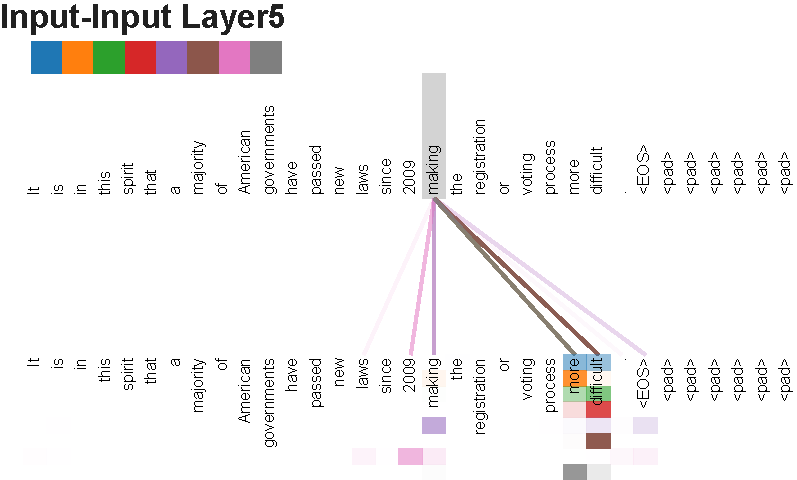
\includegraphics[width=\textwidth, trim=0 0 0 36, clip]{./vis/making_more_difficult5_new.pdf}}
\caption{An example of the attention mechanism following long-distance dependencies in the encoder self-attention in layer 5 of 6. Many of the attention heads attend to a distant dependency of the verb `making', completing the phrase `making...more difficult'.  Attentions here shown only for the word `making'. Different colors represent different heads. Best viewed in color.}
\end{figure*}

\begin{figure*}
{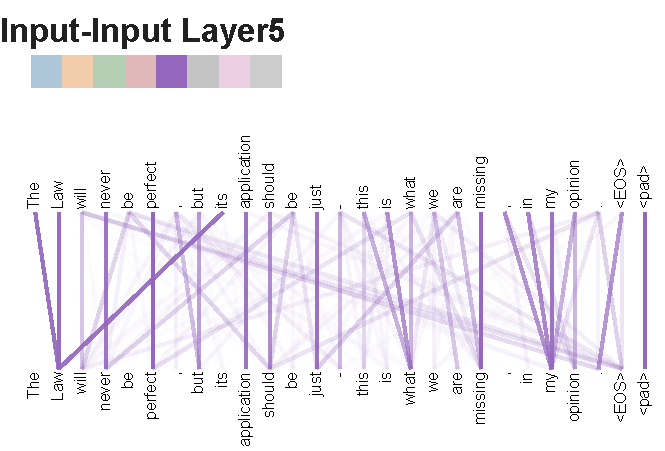
\includegraphics[width=\textwidth, trim=0 0 0 45, clip]{./vis/anaphora_resolution_new.pdf}}
{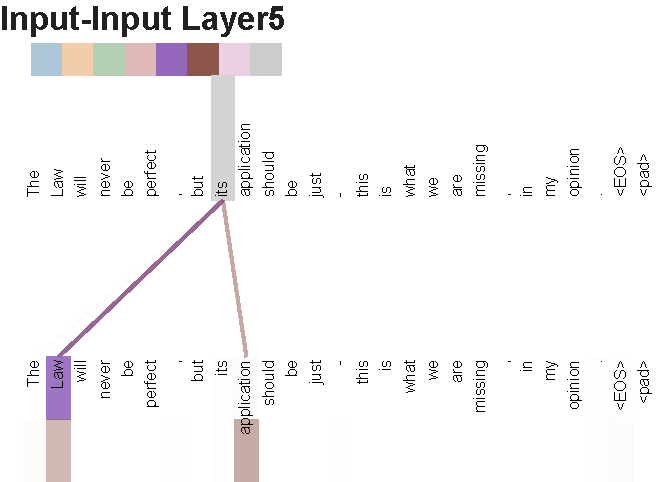
\includegraphics[width=\textwidth, trim=0 0 0 37, clip]{./vis/anaphora_resolution2_new.pdf}}
\caption{Two attention heads, also in layer 5 of 6, apparently involved in anaphora resolution. Top: Full attentions for head 5. Bottom: Isolated attentions from just the word `its' for attention heads 5 and 6. Note that the attentions are very sharp for this word.}
\end{figure*}

\begin{figure*}
{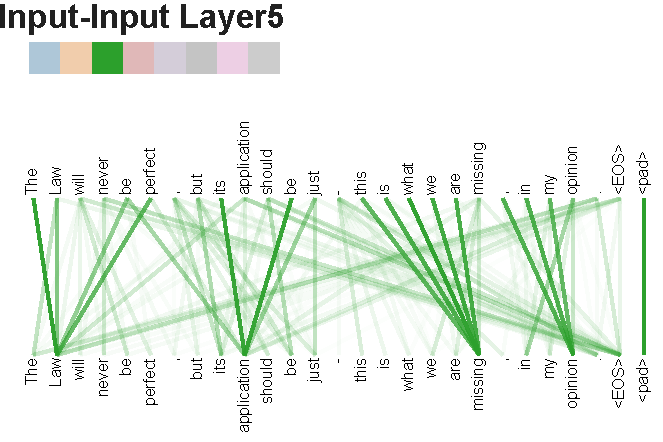
\includegraphics[width=\textwidth, trim=0 0 0 36, clip]{./vis/attending_to_head_new.pdf}}
{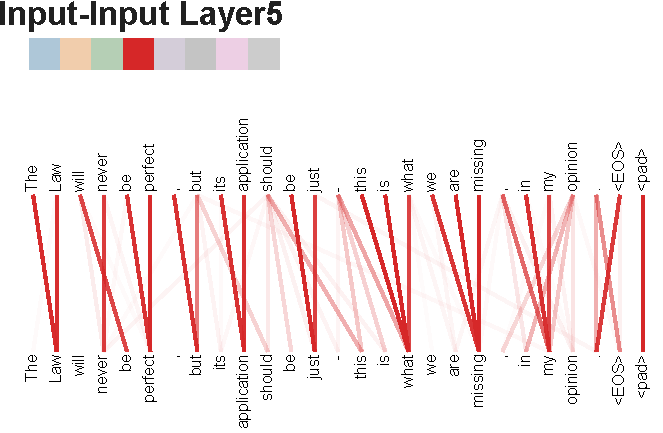
\includegraphics[width=\textwidth, trim=0 0 0 36, clip]{./vis/attending_to_head2_new.pdf}}
\caption{Many of the attention heads exhibit behaviour that seems related to the structure of the sentence. We give two such examples above, from two different heads from the encoder self-attention at layer 5 of 6. The heads clearly learned to perform different tasks.}
\end{figure*}


\end{document}